\question In the region of space shown in the figure, there is an electric field which is produced by charges that are not shown in the diagram.

\begin{center}
	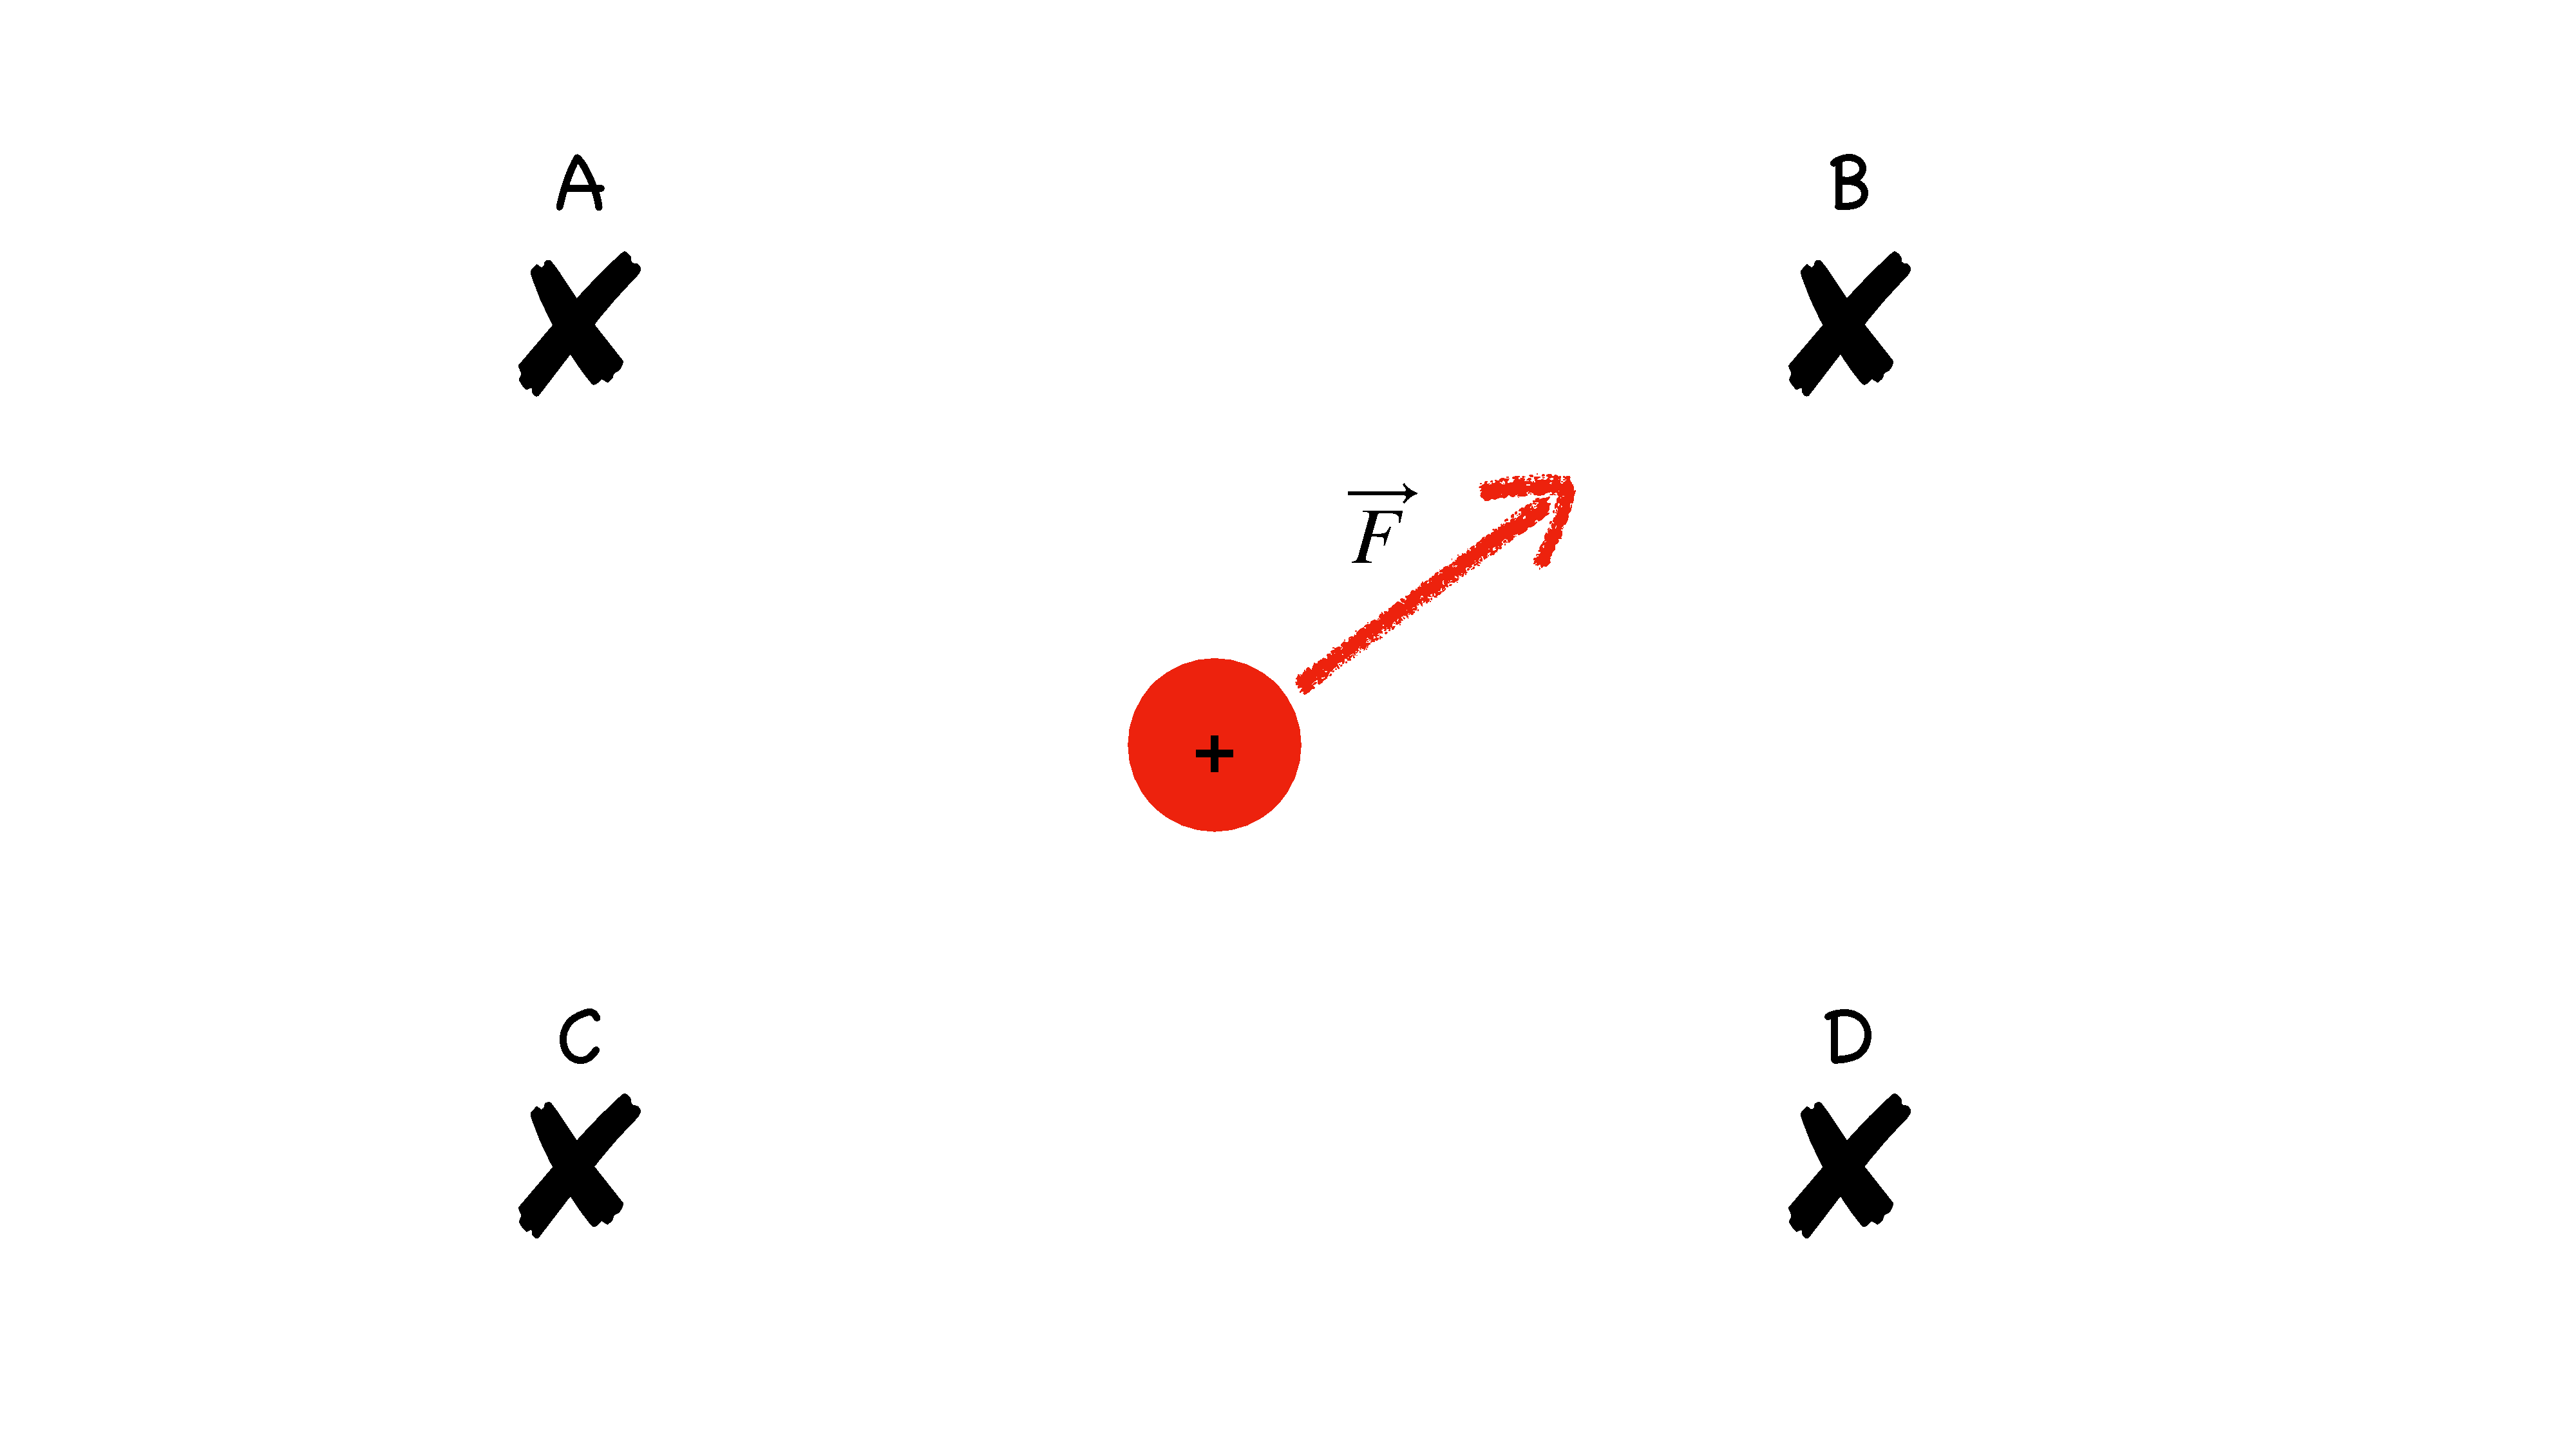
\includegraphics[width=.5\textwidth]{p3_diag1}
	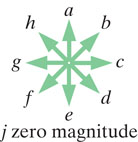
\includegraphics[width=.2\textwidth]{arrow_choice.jpg}
\end{center}

\begin{parts}
	\part The positively charged particle feels a force in the direction indicated. Which arrow (a-j) best describes the direction of the electric field vector at the location of the particle?
	\vspace{1cm}
	\part Now the positively charged particle is completely removed and replaced with a negatively charged particle. The electric field in the region is unchanged. Which arrow (a-j) best describes the direction of the force on the negatively charged particle?
	\vspace{1cm}
	\part Suppose you discover that the source of the electric field in this region is a single negatively charged particle. Which of the locations in the figure (A, B, C, or D) is a possible location for this negative charge?
\end{parts}